% mainfile: ../../../../master.tex
\subsection{AOSP Hardware Abstraction Layer}
\label{task:20231117_aosp_hal}

The interface to the hardware is a device drivers which are usually device specific and sometimes proprietary. A single set of C header files describes the functionality that a HAL provides to the Android system. HAL Code for a particular device is the implementation of the API defined by those header files, so that no code above the HAL needs to be changed to port Android to use the new device.

\subsubsection*{HAL Code Structure}

\begin{figure}[H]
    \centering
    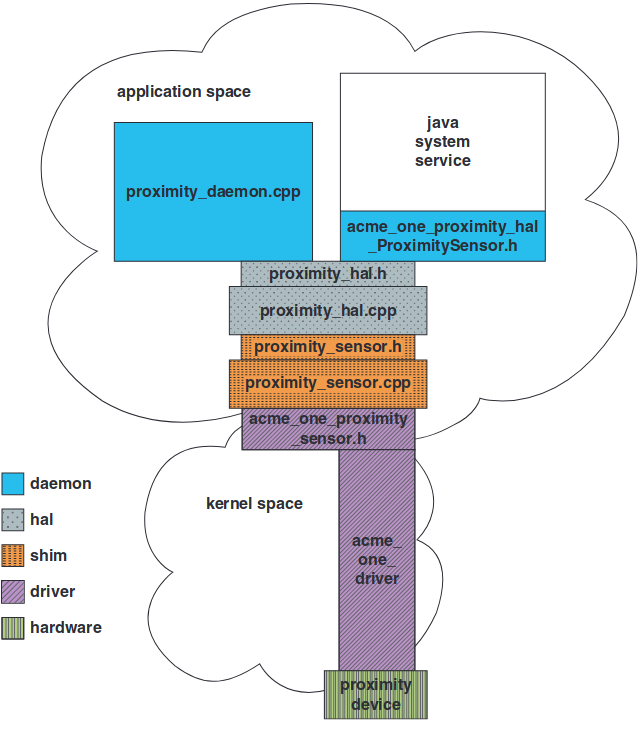
\includegraphics[width=.75\linewidth]{entries/2023/11/17/hal.png}
    \caption{HAL Layer Structure}
    \label{fig:hallayerstruct}
\end{figure}

The code consists of four functional components as show in Figure~\ref{fig:hallayerstruct}:
\begin{enumerate}
    \item \textbf{HAL code (dotted boxes):} Abstraction that separates the capabilities of hardware from its specific implementations. The \texttt{.h} file defines the HAL interface, and the implementation (\texttt{.cpp} file) specializes the Android HAL API for the target hardware. 
    \item \textbf{Shim code (dashed boxes):} Glue code that connects the HAL to a specific device hardware/driver. This code adapts the Android HAL API to the device driver for the hardware.
    \item \textbf{Daemon (blue):} Stand-alone application that interacts with the hardware through the HAL.
    \item \textbf{Java System Service (white):} System Service that Android applications will use to access the custom hardware.
\end{enumerate}

The source for those components are structured like in the directory tree below:
\dirtree{%
.1 one.
.2 app.
.2 native\_daemon.
.3 {...}.
.2 java\_daemon.
.3 {...}.
.2 proximity.
.3 include.
.4 dev.
.5 {...}.
.4 {...}.
.3 dev.
.4 {...}.
.3 hal.
.4 {...}.
.3 jni.
.4 {...}.
}
where \path{one} is the device folder of the AOSP project.  All the code implementing the HAL for the proximity sensors goes into a new subdirectory \path{proximity}.\footnote{To be a "real" HAL, the interface \path{proxmity/include/proximity_hal.h} would have to be promoted from its current directory specifically for the One device, up into the Android source tree to a location that would make it visible to other code that needed to use it. Here, it is only shared by Acme devices, so it is put under the subdirectory of the Acme device directory. If it's visible across device from multiple vendors, it might be promoted into the \path{device} directory itself.}

